\chapter{Gestenerkennung}
Handgesten gelten als Kommunikationsmittel, besonders bei gehörlosen Menschen. Sie werden auch in der kontaktlosen Interaktion mit Geräten verwendet. Dafür ist ein Ansatz nötig, um Handgesten
zu erkennen. Es wird zwischen optischen und nicht-optischen Ansätzen unterschieden. Die optischen Ansätze nutzen einen
oder mehrere Kameras, um eine Folge von Bildern aufzunehmen. Dieser Ansatz ist aber empfindlich gegenüber den vorherschenden Lichtverhältnissen.
Nicht-optische Ansätze bedienen sich anderen Sensoren, z. B. Infrarot Abstandssensoren, oder nutzen technische Hilfsmittel um zusätzliche Daten zu erfassen.
\newline
\newline
Im Bereich der optischen Handgestenerkennung auf kleinen Mikrocontrollern hat das Institut für Telematik von der Technischen Universität Hamburg Harburg (TUHH) bereits mehrere ML Ansätze untersucht.
Es konnten Gestenkandidaten zuverlässig erkannt werden und davon bis 98,98\% korrekt klassifiziert werden. Auch Nullgesten, d. h. invalide Gesten, konnten zuverlässig erkannt werden. Das verwendete neuronale Netz
benötigte 6,8 ms zur Ausführung auf dem Arduino Board ATmega328P.

\section{Ähnliche Arbeiten}
Es gibt viele Ansätze, die sich mit der Gestenerkennung beschäftigen. Es wird unterschieden zwischen optischen und nicht-optischen Ansätzen. Der optische Ansatz nutzt einen
oder mehrere Kameras um eine Folge von Bildern aufzunehmen. Dieser Ansatz ist allerdings empfindlich gegenüber Lichtverhältnisse und der Distanz die der
Nutzer zu den Kameras hat \cite{song2019design}. Nicht-optische Ansätze bedienen sich anderen Sensoren, z. B. Infrarot Abstandssensoren \cite{cheng2011contactless},
oder nutzen technische Hilfsmittel um zusätzliche Daten zu erfassen.
\newline
\newline
Song et al. \cite{song2019design} haben die Handgestenerkennung mit Gradient Boosting Entscheidungsbäumen untersucht. Sie wählten einen nicht-optischen Ansatz, der aus einen tragbaren sEMG Recorder
der die elektrischen Signale der Muskelaktivitäten erfasst. Als Eingabe für den Entscheidungsbaum wählten sie neun Features die in die Kategorie von zeitabhängigen Features einzuordnen sind
(siehe Tabelle \ref{tab:songFeatures}). Damit erzielten sie eine Erkennungsgenauigkeit von 91\% unter 12 verschiedenen Handgesten.
\begin{table}[h!]
    \centering
    \begin{tabular}{ c | c | c }
        \hline
        \hline
        1 & Mean absolute value & $\frac{1}{N}\sum^N_{t=1} |x_t|$ \\\hline
        2 & Simple square integral & $\sum^N_{t=1} |x_t|^2$ \\\hline
        3 & Minimum value & $\min x_t$ \\\hline
        4 & Maximum value & $\max x_t$ \\\hline
        5 & Standard deviation & $\sqrt{\frac{1}{N}\sum^N_{t=1}(x_t - \tilde{x})^2}$ \\\hline
        6 & Average amplitude change & $\frac{1}{N-1}\sum^{N-1}_{t=1} |x_{t + 1} - x_t|$ \\\hline
        7 & Zero crossing & $\sum^{N-1}_{t=1}diff(sgn(x_{t+1}),sgn(x_t))$ \\\hline
        8 & Slope sign change & $\sum^{N-2}_{t=1}diff(sgn(x_{t+1} - x_t),sgn(x_t - x_{t - 1}))$ \\\hline
        9 & Willison amplitude & $\sum^{N-1}_{t=1}u(|x_{t+1} - x_t| - threshold)$ \\
        \hline
        \hline
    \end{tabular}
    \caption{Die von Song et al. genutzten Features \cite{song2019design}.}
    \label{tab:songFeatures}
\end{table}
\newline
\newline
Ahad et al. \cite{ahad2012motion} diskutieren den Motion History Image (MHI) Ansatz. MHI ist ein optischer Ansatz, der eine Sequenz von Bildern in ein einziges komprimiert. Dabei werden dominate Bewegungen die
kürzlich verarbeitet wurden heller angezeigt als nicht dominate Bewegungen oder Bewegungen die schon länger zurück liegen.
\begin{align}
    H_{\tau}(x,y,t) = \begin{cases}
                          \tau & if \psi(x,y,t) = 1 \\
                          \max(0, H_{\tau}(x,y,t-1) - \delta) & otherwise
    \end{cases}
    \label{formular:mhi}
\end{align}
Das MHI kann sequentiell berechnet werden. Initial sind alle Werte 0. Wenn $\psi(x,y,t)$ eine dominate Bewegung in einem Pixel $(x,y)$ zu einem Zeitpunkt $t$ signalisiert, dann wird der Pixel zum Maximalwert $\tau$
gesetzt. Mit jedem Bild in denen keine dominate Bewegung im Pixel $(x,y)$ stattgefunden hat, wird der Wert um den Zerfallswert $\delta$ dekrementiert bis zu einem Minimum von 0 (siehe Formel \ref{formular:mhi}).
\newline
\newline
MHI ist leicht zu berechnen und Invariant zu Lichtverhältnissen. Allerdings ist die Leistung stark abhängig von $\psi$, $\tau$ und $\delta$. MHI ist besonders anfällig für Bildfolgen mit verschiedener Länge.
Jenachdem wie $\tau$ und $\delta$ gewählt sind, ist die Bewegungshistorie nicht sichtbar oder verloren gegangen.
\section{Optische Handgestenerkennung}
\label{sec:fallstudie}
\begin{figure}
    \centering
    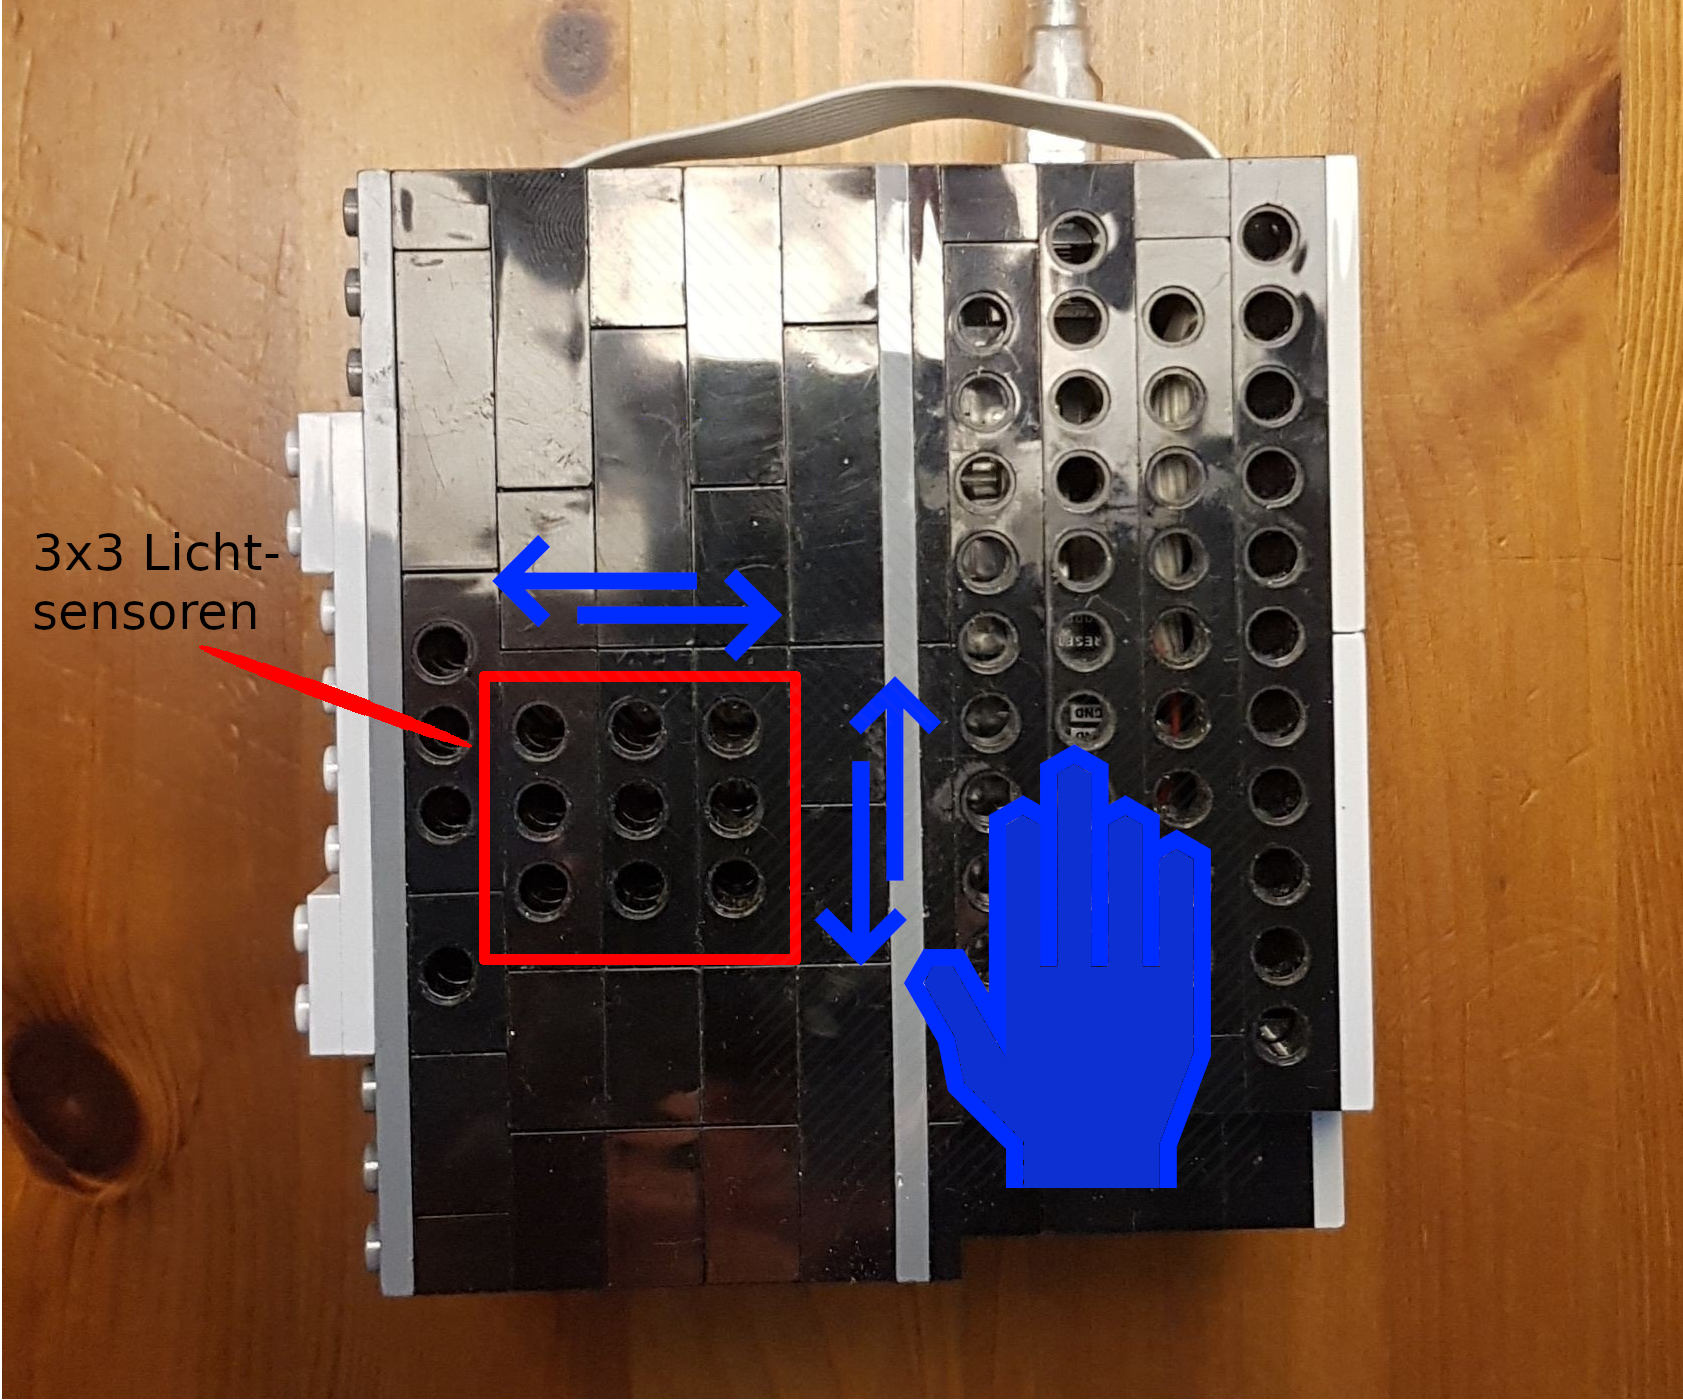
\includegraphics[width=0.6\linewidth]{images/arduino_ex.png}
    \caption{Das Arduino-Board ATmega328P mit 3x3 Matrix von Lichtsensoren in Lego-Verpackung. Illustriert werden die möglichen Handgestentypen mit Ausnahme der Nullgeste.}
    \label{fig:arduino_ex}
\end{figure}
Diese Arbeit ist Teil einer Fallstudie zur Handgestenerkennung auf Low-End Mikrocontrollern von dem Institut für Telematik an der TUHH \cite{venzkeArticle}. Das Ziel ist die Handgestenerkennung in Echtzeit mit so wenig
Ressourcen wie möglich, damit die Produktion der einzelnen Module so kostengünstig wie möglich ist. Als Eingabe dient, je nach Modul, eine 3x3, bzw. 4x4, Matrix von Lichtsensoren. Abbildung \ref{fig:arduino_ex}
illustriert 4 Typen von Handgesten, die über den Mikrocontroller ausgeführt werden: Links nach Rechts, Rechts nach Links, Oben nach Unten, Unten nach Oben. Zudem wird zwischen Handgesten und Nullgesten, d. h.
invalide Handgesten, unterschieden. In den bisherigen Arbeiten wurden ML Modelle mit künstlichen neuronalen Netzwerken erstellt. Dessen Prozessablauf zur Handgestenerkennung lässt sich auf 3
Schritte zusammenfassen.
\begin{enumerate}
    \item Extrahiere einen Gestenkandidaten.
    \item Vorverarbeite den Gestenkandidaten.
    \item Wende das Modell auf den vorverarbeiteten Gestenkandidaten an.
\end{enumerate}

\subsection{Exrahierung von Gestenkandidaten}
Die Lichtsensorenmatrix liefert einen kontinuierlichen Strom an Bildern. Dabei limitiert die Verarbeitungszeit eines Bildes die Anzahl an Bilder pro Sekunde. Als Gestenkandidat wird eine Folge von Bildern definiert, die
ein Ereignis einschließt. In diesem Fall wird das Ereignis durch die Veränderung im gleitenden Mittelwert der Lichtverhältnisse definiert, i. e. sobald der gleitende Mittelwert unterschritten wird ein Gestenkandidat
angefangen aufgenommen zu werden und sobald die Lichtverhältnisse zu dem Wert zurückkehren wird die Aufnahme beendet. Der gleitende Mittelwert wird dabei immer angepasst, wenn kein Gestenkandidat aufgenommen wird, um
sich den veränderden Lichtverhältnissen anzupassen. Da leichte Veränderungen natürlich sind, muss eine Toleranzgrenze von 10\% unterschritten werden, damit die Aufnahme gestartet wird. Dies hat als Folge, dass der Anfang
und das Ende nicht vollständig ist. Aus diesem Grund schlug Kubik zusätzlich vor am Anfang und Ende weitere Bilder anzufügen \cite{kubikThesis}.
\newline
\newline
\begin{figure}
    \usetikzlibrary{arrows,automata,positioning}
    \centering
    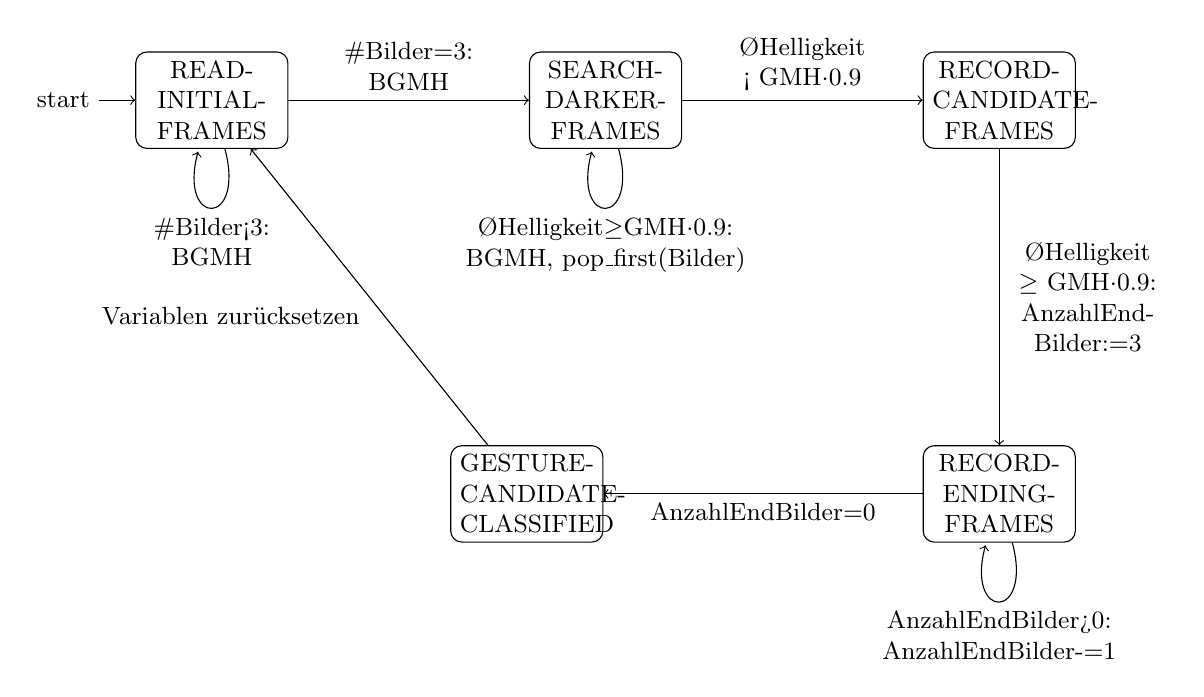
\begin{tikzpicture}[
        block/.style={
        draw,
        fill=white,
        text width=0.14*\columnwidth,
        anchor=west,
        minimum height=1cm,
        rounded corners
        },
        font=\small,
        on grid, auto,
        node distance=5cm
    ]
        \node [block,align=center,initial] (s0) {READ-INITIAL-FRAMES};
        \node [block,align=center] (s1) [right of=s0] {SEARCH-DARKER-FRAMES};
        \node [block,align=center] (s2) [right of=s1] {RECORD-CANDIDATE-FRAMES};
        \node [block,align=center] (s3) [below of=s2] {RECORD-ENDING-FRAMES};
        \node [block,align=center, node distance=6cm] (s4) [left of=s3] {GESTURE-CANDIDATE-CLASSIFIED};
        \path [->, text width=2cm, align=center] (s0) edge [loop below] node {\#Bilder<3: BGMH} (s0);
        \path [->, text width=2cm, align=center] (s0) edge node {\#Bilder=3: BGMH} (s1);
        \path [->, text width=4cm, align=center] (s1) edge [loop below] node {ØHelligkeit$\geq$GMH$\cdot 0.9$: BGMH, pop\_first(Bilder)} (s1);
        \path [->, text width=3cm, align=center] (s1) edge node {ØHelligkeit < GMH$\cdot 0.9$} (s2);
        \path [->, text width=2cm, align=center] (s2) edge node {ØHelligkeit $\geq$ GMH$\cdot 0.9$: AnzahlEndBilder:=3} (s3);
        \path [->, text width=3cm, align=center] (s3) edge [loop below] node {AnzahlEndBilder>0: AnzahlEndBilder-=1} (s3);
        \path [->, text width=3cm, align=center] (s3) edge node {AnzahlEndBilder=0} (s4);
        \path [->] (s4) edge node {Variablen zurücksetzen} (s0);
    \end{tikzpicture}
    \caption{Implementierung von Kubik's Algorithmus um Gestenkandidaten zu erkennen von Dr. Marcus Venzke. BGMH steht für die Aktion \glqq \textbf{B}erechnung \textbf{G}leitender \textbf{M}ittelwert der \textbf{H}elligkeit\grqq und GMH steht für die Variable \glqq \textbf{G}leitender \textbf{M}ittelwert der \textbf{H}elligkeit\grqq.}
    \label{fig:venzkeAlgoImpl}
\end{figure}
Abbildung \ref{fig:venzkeAlgoImpl} zeigt die konkrete Implementierung dieses Algorithmus mit einem Zustandsautomaten von Dr. Marcus Venzke. In jedem Zustand wird das aktuelle Bild dem Puffer angefügt. Der Automat
verbleibt im Zustand \texttt{READ-INITIAL-FRAMES} bis der Puffer 3 Bilder enthält und passt stets den gleitenden Mittelwert der Helligkeit an. Anschließend geht der Automat in den Zustand
\texttt{SEARCH-DARKER-FRAMES} über, indem er weiterhin den gleitenden Mittelwert anpasst und immer das erste Bild aus dem Puffer entfernt, da lediglich 3 Bilder jeweils vorm Aufnehmen und nach dem Aufnehmen des
Gestenkandidates angefügt werden sollen. Sobald die Durchschnittshelligkeit den 90\% des gleitenden Mittelwerts unterschreitet wird die Aufnahme begonnen. Der Automat geht in den Zustand \texttt{RECORD-CANDIDATE-FRAMES}
über. Dort verbleibt der Automat solange bis die Durchschnittshelligkeit 90\% des gleitenden Mittelwerts überschreitet, woraufhin der Automat in den Zustand \texttt{RECORD-ENDING-FRAMES} über geht, indem die letzten 3
Bilder an den Puffer angehängt werden. Der Zustand des Puffers im Zustand \texttt{GESTURE-CANDIDATE-CLASSIFIED} repräsentiert den Gestenkandidaten. Zuletzt werden alle nötigen Variablen zurückgesetzt und der
Automat geht in den initialen Zustand wieder über.
\section{Skalieren des Gestenkandidaten}
\label{sec:scaling}
Ein Gestenkandidat besteht aus einer variablen Anzahl von Bildern. Durch die künstlich angefügten Bilder am Anfang und Ende sind es mindestens acht Bilder. Kubik erkannte, dass ein neuronales Netz eine feste Anzahl an
Eingaben benötigt und diskutierte verschiedene Ansätze, um mit einer variablen Länge des Input umzugehen. Er verwarf die Idee den Puffer mit irrelevanten Bildern oder Nullen auszufüllen, Bilder zu duplizieren
oder Teile des Gestenkandidaten zu verwerfen. Er befürchtete, dass dadurch nicht die vollständige Handgeste auf die Eingangs-Ebene des neuronalen Netzes (NN) abgebildet werden würde, oder dass die Handgeste
womöglich verzerrt wäre \cite{kubikThesis}.
\newline
\newline
Kubik schlug vor, dass lineare Interpolation angewendet werden soll. Dabei werden die vorhandenen Bilder uniform auf 20 Pseudoindexe verteilt, sodass das erste und letzte Bild auch
jeweils den ersten und letzten Pseudoindex einnimmt. Die übrigen Indize sind gleich verteilt. Aus diesem Grund ergeben sie nicht immer natürliche Zahlen. In diesem Fall wird das Bild durch Interpolation des
vorherigen Bildes und des nächsten Bildes erzeugt. Dieser Ansatz wurde auch von Giese aufgegriffen, der sich in diesem Zusammenhang
ebenfalls mit künstlichen neuronalen Netzen beschäftigt hatte \cite{gieseThesis}.
\subsection{Trainingsdaten}
\subsection{Gestenerkennung mit künstliche neuronalen Netzen}
Insgesamt gingen dieser Arbeit 4 Arbeiten voraus, die sich mit künstlichen neuronalen Netzen im Zusammenhang dieser Fallstudie beschäftigt hatten.

\subsubsection{Engelhardt}
Engelhardt führte die in \ref{sec:fallstudie} definierten Handgesten mit der Hand, einem Finger und 2 Finger unter verschiedenen Helligkeiten aus, auf Basis dessen seine Modelle trainiert und validiert wurden. Er
argumentiert, dass rekurrente neuronale Netze (RNN), Feedforward neuronale Netze (FFNN) und Long-Short-Term Memory neuronale Netze (LSTMNN) am besten geeignet für temporale Probleme seien. Convolutional neuronale
Netze (CNN) verwarf Engelhardt aufgrund der geringen Auflösung der Gesten und da die Faltung extrem Rechenaufwendig sei. Desweiteren verwarf er LSTMNN, da diese zu viel Rechenleistung und Speicherplatz
benötigen. Als Eingabewerte zu seinen RNNs und FFNNs diente eine Sequenz von 20 Bilder die zu 180 Werten konkatiniert wurden und auf Werte zwischen 0 und 1 normalisiert wurden. Als bestes Model stellte sich eines
seiner FFNNs heraus, das auf seinen Testdaten bis zu 99\% Erkennungsgenauigkeit erzielte. Außerdem erwies es sich als robust gegenüber Rauschen und Helligkeitsveränderungen im Vergleich zum RNN. Die Ausführungszeit
des FFNN belief sich auf 11,54 ms mit einem Verbrauch von 11 kB Flash-Speicher und 573 bytes RAM \cite{engelhardtThesis}.

\subsubsection{Kubik}

\subsubsection{Klisch}

\subsubsection{Giese}
